\documentclass[sigplan,10pt]{acmart}

\usepackage[utf8]{inputenc}
\usepackage{listings}
\usepackage{todonotes}
\usepackage{comment}    % comments.
\usepackage{url}    % url.

\settopmatter{printfolios=true}

\graphicspath{{./data/img/}}

% Copyright
%\setcopyright{none}
%\setcopyright{acmcopyright}
%\setcopyright{acmlicensed}
\setcopyright{rightsretained}
%\setcopyright{usgov}
%\setcopyright{usgovmixed}
%\setcopyright{cagov}
%\setcopyright{cagovmixed}


% DOI
%\acmDOI{10.475/123_4}

% ISBN
%\acmISBN{123-4567-24-567/08/06}

%Conference
\acmConference[SEPS 2017]{4th International Workshop on Software Engineering for Parallel Systems}{October 2017}{Vancouver, Canada}
\acmYear{2017}
\copyrightyear{2017}

%\acmPrice{15.00}

%\acmBadgeL[http://ctuning.org/ae/ppopp2016.html]{ae-logo}
%\acmBadgeR[http://ctuning.org/ae/ppopp2016.html]{ae-logo}



\begin{document}
%---
\title{Comparing OpenMP and PThreads}
%\titlenote{...}
\subtitle{from the learning aspects to the real performance results}
%\subtitlenote{...}
%---
\author{Pedro Bruel}
%\authornote{This author is the one who did all the really hard work.}
\affiliation{%
  \institution{Software Systems Laboratory (LSS)\\ Institute of Mathematics and Statistics\\ University of São Paulo}
  \streetaddress{Rua do Matão, 1010}
  \city{São Paulo}
  \country{Brazil}
  \postcode{05508-090}
}
\email{phrb@ime.usp.br}
%---
\author{Raphael Cobe}
%\authornote{Ph.D.}
\affiliation{%
  \institution{Núcleo de Computação Científica \\ Universidade Estadual Paulista}
  \streetaddress{...}
  \city{São Paulo}
  \country{Brazil}
  \postcode{...}
}
\email{rmcobe@ncc.unesp.br}
%---
\author{Alfredo Goldman}
%\authornote{Professor: the head.}
\affiliation{%
  \institution{Software Systems Laboratory (LSS)\\ Institute of Mathematics and Statistics\\ University of São Paulo}
  \streetaddress{Rua do Matão, 1010}
  \city{São Paulo}
  \country{Brazil}
  \postcode{05508-090}
}
\email{gold@ime.usp.br}

%---

\renewcommand{\shortauthors}{Bruel et al.}

%--
\begin{abstract}
TO-DO ...
\end{abstract}

%---

\maketitle

%---
\section{Introduction}
\label{sec:introduction}

...

In this context, the approach of using Compilation Directives to guide the
compiler in the parallelization process has gained popularity. These directives
are implemented using the compiler's pre-processing directives and are utilized
as annotations that provide tips about the sequential code. Among the tools and
extensions that use compilation directives are the \texttt{OpenMP} API
\cite{Dagum1998a} \cite{Chapman:2007} used for writing programs for multi-core
architectures, and the \texttt{OpenACC} programming
standard~\cite{openacc:api}, used for writing programs for heterogeneous
CPU/GPU architectures. The \texttt{OpenMP 4.0} specification supports
offloading capabilities \cite{openmp:api:2013} such as \texttt{OpenACC} and
\texttt{AMD HSA}~\cite{amd:hsa:site}. These tools aim to make easier the task
of designing and implementing efficient and provably correct parallel
algorithms. However, the abstraction layers built by the extensions also have
the potential to conceal architectural details and to generate new parallel
programming challenges.

When comparing \texttt{OpenMP} to other available tools for developing
multi-threaded applications such as the \texttt{pthreads} interface, the API
can be considered almost costless. However, when writing more complex
applications this may not be true. The design and implementation of such
complex applications require more knowledge about platforms and execution
models than what can be shown by tutorials, that present high level and trivial
examples. These tutorials try to convince the user that programming with
directives is simple and easy to do, which is not always true. For instance, to
achieve good performance in some cases it is necessary to describe many
restrictions on annotations~\cite{OpenMPTasks2009}~\cite{mattson2003good}.

Krawezik and Cappello~\cite{CPE:CPE905} evidenced this difficulty by comparing
MPI and three OpenMP versions of benchmarks. The most popular use of
\texttt{OpenMP} directives is at the loop level. The programmer discovers
potentially parallel loops and annotates the code with directives starting and
closing parallel regions. Good results were obtained only when SPMD was
implemented on OpenMP, and achieving good performance required a significant
programming effort~\cite{CPE:CPE905}.

In this work we have gathered data from assignments made by graduate students
for the \emph{Introduction to Parallel and Distributed Computing} course. Among
other exercises, the students were asked to find examples of \texttt{OpenMP}
code in tutorials and official manuals that failed under special conditions.
These conditions could be created by, for example, placing barriers or forcing
racing conditions by exposing inaccurate thread management.


The rest of the paper is organized as follows. The following section discusses
related work... 


\section{Background}
\label{sec:background}

%\todo[inline,color=cyan,author=Pedro]{Cite our previous paper, making it clear that we are the authors}
%\todo[inline,color=cyan,author=Pedro]{Describe related work}
%\todo[inline,color=cyan,author=Pedro]{Describe related work since last paper}

The selection of teaching tools for Parallel and Distributed classes impacts
the development of students' abilities to solve algorithmic problems
efficiently. The importance of selecting good tools for teaching Parallel and
Distributed Computing has been increasingly important, especially since the
topic became a core component of the ACM undergraduate computer science
curricula in 2013~\cite{acmcurricula}.

Different approaches have been used to study the selection of the best level of
abstraction for teaching Parallel and Distributed programming courses.
Falcao~\cite{6565518} argues that introducing a high-level parallel programming
interface such as \textit{OpenMP} in the beginning of an undergraduate computer
science course would cause a small overhead and benefit the rest of the course.
Foley \textit{et al.}~\cite{FOLEY2017138} support the introduction of practical
learning experiences along an undergraduate course, of increasing depth as the
course progresses. They introduce OnRamp, a web application to help students
learn to write parallel code starting with practical and moving to conceptual
experiences.  Pllana \textit{et al.}~\cite{Pllana:2009} adopt a Model Driven
Development approach to develop parallel solutions using Parallel Building
Blocks. They introduce a programming environment that transforms these
high-level models in source code. The tool's goal is to hide from the students
the complexity of writing parallel code.

The approaches mentioned so far introduce tools for parallel programming before
the related concepts.  Other approaches instead consider learning software
tools as just one of the objectives of the course, and argue that their
introduction should come after the introduction of concepts of Parallel and
Distributed Computing.

In previous work~\cite{goncalves:OpenMPNotEasy} we show that teaching the
concepts of parallel programming first instead of high-level parallel
programming APIs is important, especially because the available resources and
tutorials for these APIs may contain difficult to find errors.  We listed
several sources of tutorials and hands-on materials obtained in the internet in
which undergraduate students were able to point parallel correctness
errors~\cite{SuB:2005:CMO:1892830.1892863}.

Sü\ss{} and Leopold~\cite{Leopold:userOpenMP} discuss the inability to express
all parallel solutions in tools such as \textit{OpenMP}. They used a sorting
algorithm to show that it is easy to find patterns that are difficult to
implement in \textit{OpenMP}, but can be easily implemented in lower-level
programming interfaces, such as POSIX Threads.

Adams~\cite{ADAMS201731} presented a set of patterns implemented using
\textit{Pthreads} that can help students understand aspects of parallel
programming that would be difficult to grasp using only \textit{OpenMP}
examples. His catalog also contained patterns implemented in \textit{OpenMP}.

\todo[inline,color=cyan,author=Pedro]{This last paragraph maybe fits best in
the end of the introduction}

In this paper we present data that supports the importance of composing a
curriculum for Parallel and Distributed Computing courses using low-level
programming interfaces, such as \textit{Pthreads}, as well as high-level
interfaces, such as \textit{OpenMP}.  Brown \textit{et
al.}~\cite{Brown:2010:SPC:1971681.1971689}, points that the choice of a
software tool should be only one of the topics explored during a parallel
programming course. Topics such as data structures, algorithms, software design
and parallel hardware platforms should also be explored.

\todo[inline,color=orange,author=Raphael]{Maybe we should make a better
connection between the end of this section and the next one;}

\section{Related Work}
\label{sec:relatedwork}

%\todo[inline,color=cyan,author=Pedro]{Cite our previous paper, making it clear that we are the authors}
%\todo[inline,color=cyan,author=Pedro]{Describe related work}
%\todo[inline,color=cyan,author=Pedro]{Describe related work since last paper}

The selection of teaching tools for Parallel and Distributed classes impacts
the development of students' abilities to solve algorithmic problems
efficiently. The importance of selecting good tools for teaching Parallel and
Distributed Computing has been increasingly important, especially since the
topic became a core component of the ACM undergraduate computer science
curricula in 2013~\cite{acmcurricula}.

Different approaches have been used to study the selection of the best level of
abstraction for teaching Parallel and Distributed programming courses.
Falcao~\cite{6565518} argues that introducing a high-level parallel programming
interface such as \textit{OpenMP} in the beginning of an undergraduate computer
science course would cause a small overhead and benefit the rest of the course.
Foley \textit{et al.}~\cite{FOLEY2017138} support the introduction of practical
learning experiences along an undergraduate course, of increasing depth as the
course progresses. They introduce OnRamp, a web application to help students
learn to write parallel code starting with practical and moving to conceptual
experiences.  Pllana \textit{et al.}~\cite{Pllana:2009} adopt a Model Driven
Development approach to develop parallel solutions using Parallel Building
Blocks. They introduce a programming environment that transforms these
high-level models in source code. The tool's goal is to hide from the students
the complexity of writing parallel code.

The approaches mentioned so far introduce tools for parallel programming before
the related concepts.  Other approaches instead consider learning software
tools as just one of the objectives of the course, and argue that their
introduction should come after the introduction of concepts of Parallel and
Distributed Computing.

In previous work~\cite{goncalves:OpenMPNotEasy} we show that teaching the
concepts of parallel programming first instead of high-level parallel
programming APIs is important, especially because the available resources and
tutorials for these APIs may contain difficult to find errors.  We listed
several sources of tutorials and hands-on materials obtained in the internet in
which undergraduate students were able to point parallel correctness
errors~\cite{SuB:2005:CMO:1892830.1892863}.

Sü\ss{} and Leopold~\cite{Leopold:userOpenMP} discuss the inability to express
all parallel solutions in tools such as \textit{OpenMP}. They used a sorting
algorithm to show that it is easy to find patterns that are difficult to
implement in \textit{OpenMP}, but can be easily implemented in lower-level
programming interfaces, such as POSIX Threads.

Adams~\cite{ADAMS201731} presented a set of patterns implemented using
\textit{Pthreads} that can help students understand aspects of parallel
programming that would be difficult to grasp using only \textit{OpenMP}
examples. His catalog also contained patterns implemented in \textit{OpenMP}.

\todo[inline,color=cyan,author=Pedro]{This last paragraph maybe fits best in
the end of the introduction}

In this paper we present data that supports the importance of composing a
curriculum for Parallel and Distributed Computing courses using low-level
programming interfaces, such as \textit{Pthreads}, as well as high-level
interfaces, such as \textit{OpenMP}.  Brown \textit{et
al.}~\cite{Brown:2010:SPC:1971681.1971689}, points that the choice of a
software tool should be only one of the topics explored during a parallel
programming course. Topics such as data structures, algorithms, software design
and parallel hardware platforms should also be explored.

\todo[inline,color=orange,author=Raphael]{Maybe we should make a better
connection between the end of this section and the next one;}

\section{Research Design}
\label{sec:researchdesign}

This section describes our research design. We devised a questionnaire
regarding student experience with solving the same problem using
\textit{Pthreads} and \textit{OpenMP} during the Concurrent, Parallel and
Distributed Computing Course at the Computer Science program of the University
of São Paulo. We answered 3 research questions analysing the students'
responses.

\subsection{The Course}

The Computer Science program of the University of São Paulo offers Concurrent,
Parallel and Distributed Computing courses for graduate and undergraduate
students in a single class. The course aims to promote meaningful exchanges of
knowledge and experience between undergraduate and graduate students.

The course presents students with a series of software engineering challenges
in the form of assignments involving GPU programming with CUDA and distributed
computing with OpenMPI. The final is composed of an essay and a presentation on
a relevant topic related to Concurrent, Parallel and Distributed Computing.
The course material is available
online~\footnote{\url{https://phrb.github.io/MAC5742-0219} [Accessed in
07/08/2017]}.

We devised an assignment to measure the students' difficulties to learn and use
\textit{Pthreads} and \textit{OpenMP} to solve a simple problem. Students had
to form groups of 2 to 3 members and implement parallel versions of a
sequential code using \textit{Pthreads} and \textit{OpenMP}.  We provided a
sequential implementation for the calculation of the Mandelbrot
Set~\cite{douady1984etude}. The sequential code presented an embarrassingly
parallel problem with two nested loops, and a third loop with dependent
iterations that could not be parallelized easily.

\begin{figure}[htb]
\begin{minipage}{\linewidth}
\begin{lstlisting}[language=C, basicstyle=\ttfamily\scriptsize, numbers=left,
                   frame=no, showspaces=false, showstringspaces=false,
                   numberstyle=\tiny,
                   xleftmargin=0.5cm,
                   keywords={%
                       DATATYPE, pthread_t, pthread_create,
                       pthread_join, task_function, NULL, int, main,
                       void, printf, return, pthread_mutex_t,
                       pthread_attr_t, pthread_attr_init,
                       MAX_THREADS, SIZE, char, struct, malloc,
                       MIN, pthread_mutex_lock, pthread_mutex_unlock,
                       pthread_exit, from, to, and%
                       },
                   otherkeywords={::, \#pragma, \#include, <<<,>>>, \&, \*, +, -, /, [, ], >, <}
                   ]
z = 0;
for(x from 0 to x_max - 1) {
    /* Independent iterations */
    for(y from 0 to y_max - 1) {
        /* Independent iterations */
        for (iteration from 0 to iteration_max,
             and f_c(z) < limit) {
            /* Iterations depend on
               previous values of z */
            z = f_c(z);
        }
    }
}
\end{lstlisting}
\end{minipage}
\caption{Pseudocode for the computation of the Mandelbrot set}
\label{lst:mandelbrot-pseudo}
\end{figure}

The Mandelbrot set is informally defined as the set of complex numbers $c$ for
which the function $f_c(z) = z^2 + x$ does not diverge when iterated starting
in $z=0$, that is, the sequence the sequence $f_c(0), f_c(f_c(0)),
f_c(f_c(f_c(0))),\dots$ is always limited. Figure~\ref{lst:mandelbrot-pseudo}
shows pseudocode for the computation of the Mandelbrot set, listing which loops
have dependent and independent iterations.

The assignment required that the students measure the performance of the
sequential code and the performance improvements they achieved using
\textit{Pthreads} and \textit{OpenMP}. After completing the assignment we asked
the students to answer a questionnaire.

\subsection{Questionnaire}

After students organized themselves in groups of 2 to 3 students and designed
and implemented their parallel versions of the code, each individual student
was asked to answer a questionnaire. The questionnaire had two parts. The first
part asked questions about the students' previous experiences with common
programming languages and parallel and distributed programming concepts and
tools. We were also interested in students' perception of the impact of our
classes on \textit{Pthreads} and \textit{OpenMP} on their learning difficulty.

The questions of the second part were related to the students'
experience with \textit{Pthreads} and \textit{OpenMP} after
the completion of the assignment.

We obtained the ethical approval from the Department of Computer Science at the
University of São Paulo to conduct this study based on the questionnaire. We
collected responses, and consent to use them in our research, from 38 of the 54
students enrolled in the Concurrent, Parallel and Distributed Computing course.
Section \ref{sec:responses} presents a detailed description of each set of
questions and our analysis of the students' responses.

\subsection{Research Questions}
\label{sec:resques}

In previous work~\cite{goncalves:OpenMPNotEasy} we showed that teaching
\textit{OpenMP} requires the introduction of important parallel and distributed
computing concepts first, since it is easy to find errors on commonly used
\textit{OpenMP} learning material.

In this paper we argue that students are capable of learning and using
\textit{Pthreads} to obtain good performance improvements, despite their
perception that \textit{OpenMP} is much easier to learn and use.
The research questions that led the development of the questionnaire
and our analysis of the students' responses were the following:

\begin{description}
    \item[RQ1:] \textit{According to the students' perception, which API was
        easier to learn and use?}
    \item[RQ2:] \textit{With which API did the students improve performance the
        most?}
    \item[RQ3:] \textit{Did the students' performance improvements match their
        perception?}
\end{description}

To answer the first two questions we used students' responses to
our questionnaire. To answer the third question we analysed the
students' submissions and parallel implementations. The
students' responses and our analysis are presented next.

\section{Students' Background \& Responses}
\label{sec:responses}

In this section we present the background of our students in the technologies
relevant to the course and to the assignment. Then we present the responses
given by the students to our questionnaire. The questions are listed in Tables
\ref{tab:likert} and \ref{tab:comparisons}.

\todo[inline,color=cyan,author=Pedro]{Improve figure colorscheme}

\subsection{Background}

The course of Concurrent, Parallel and Distributed Computing is offered to
students of both the graduate and undergraduate programs in Computer Science at
the University of São Paulo. To gauge the proficiency and knowledge of our
students we elaborated a five-point scale from \textit{Do not Know} $(1)$ to
\textit{Expert or Proficient} $(5)$.  We asked the students to express their
proficiency level on this scale, and their responses are shown in Figure
\ref{fig:background}.

\begin{figure}[htpb]
    \centering
    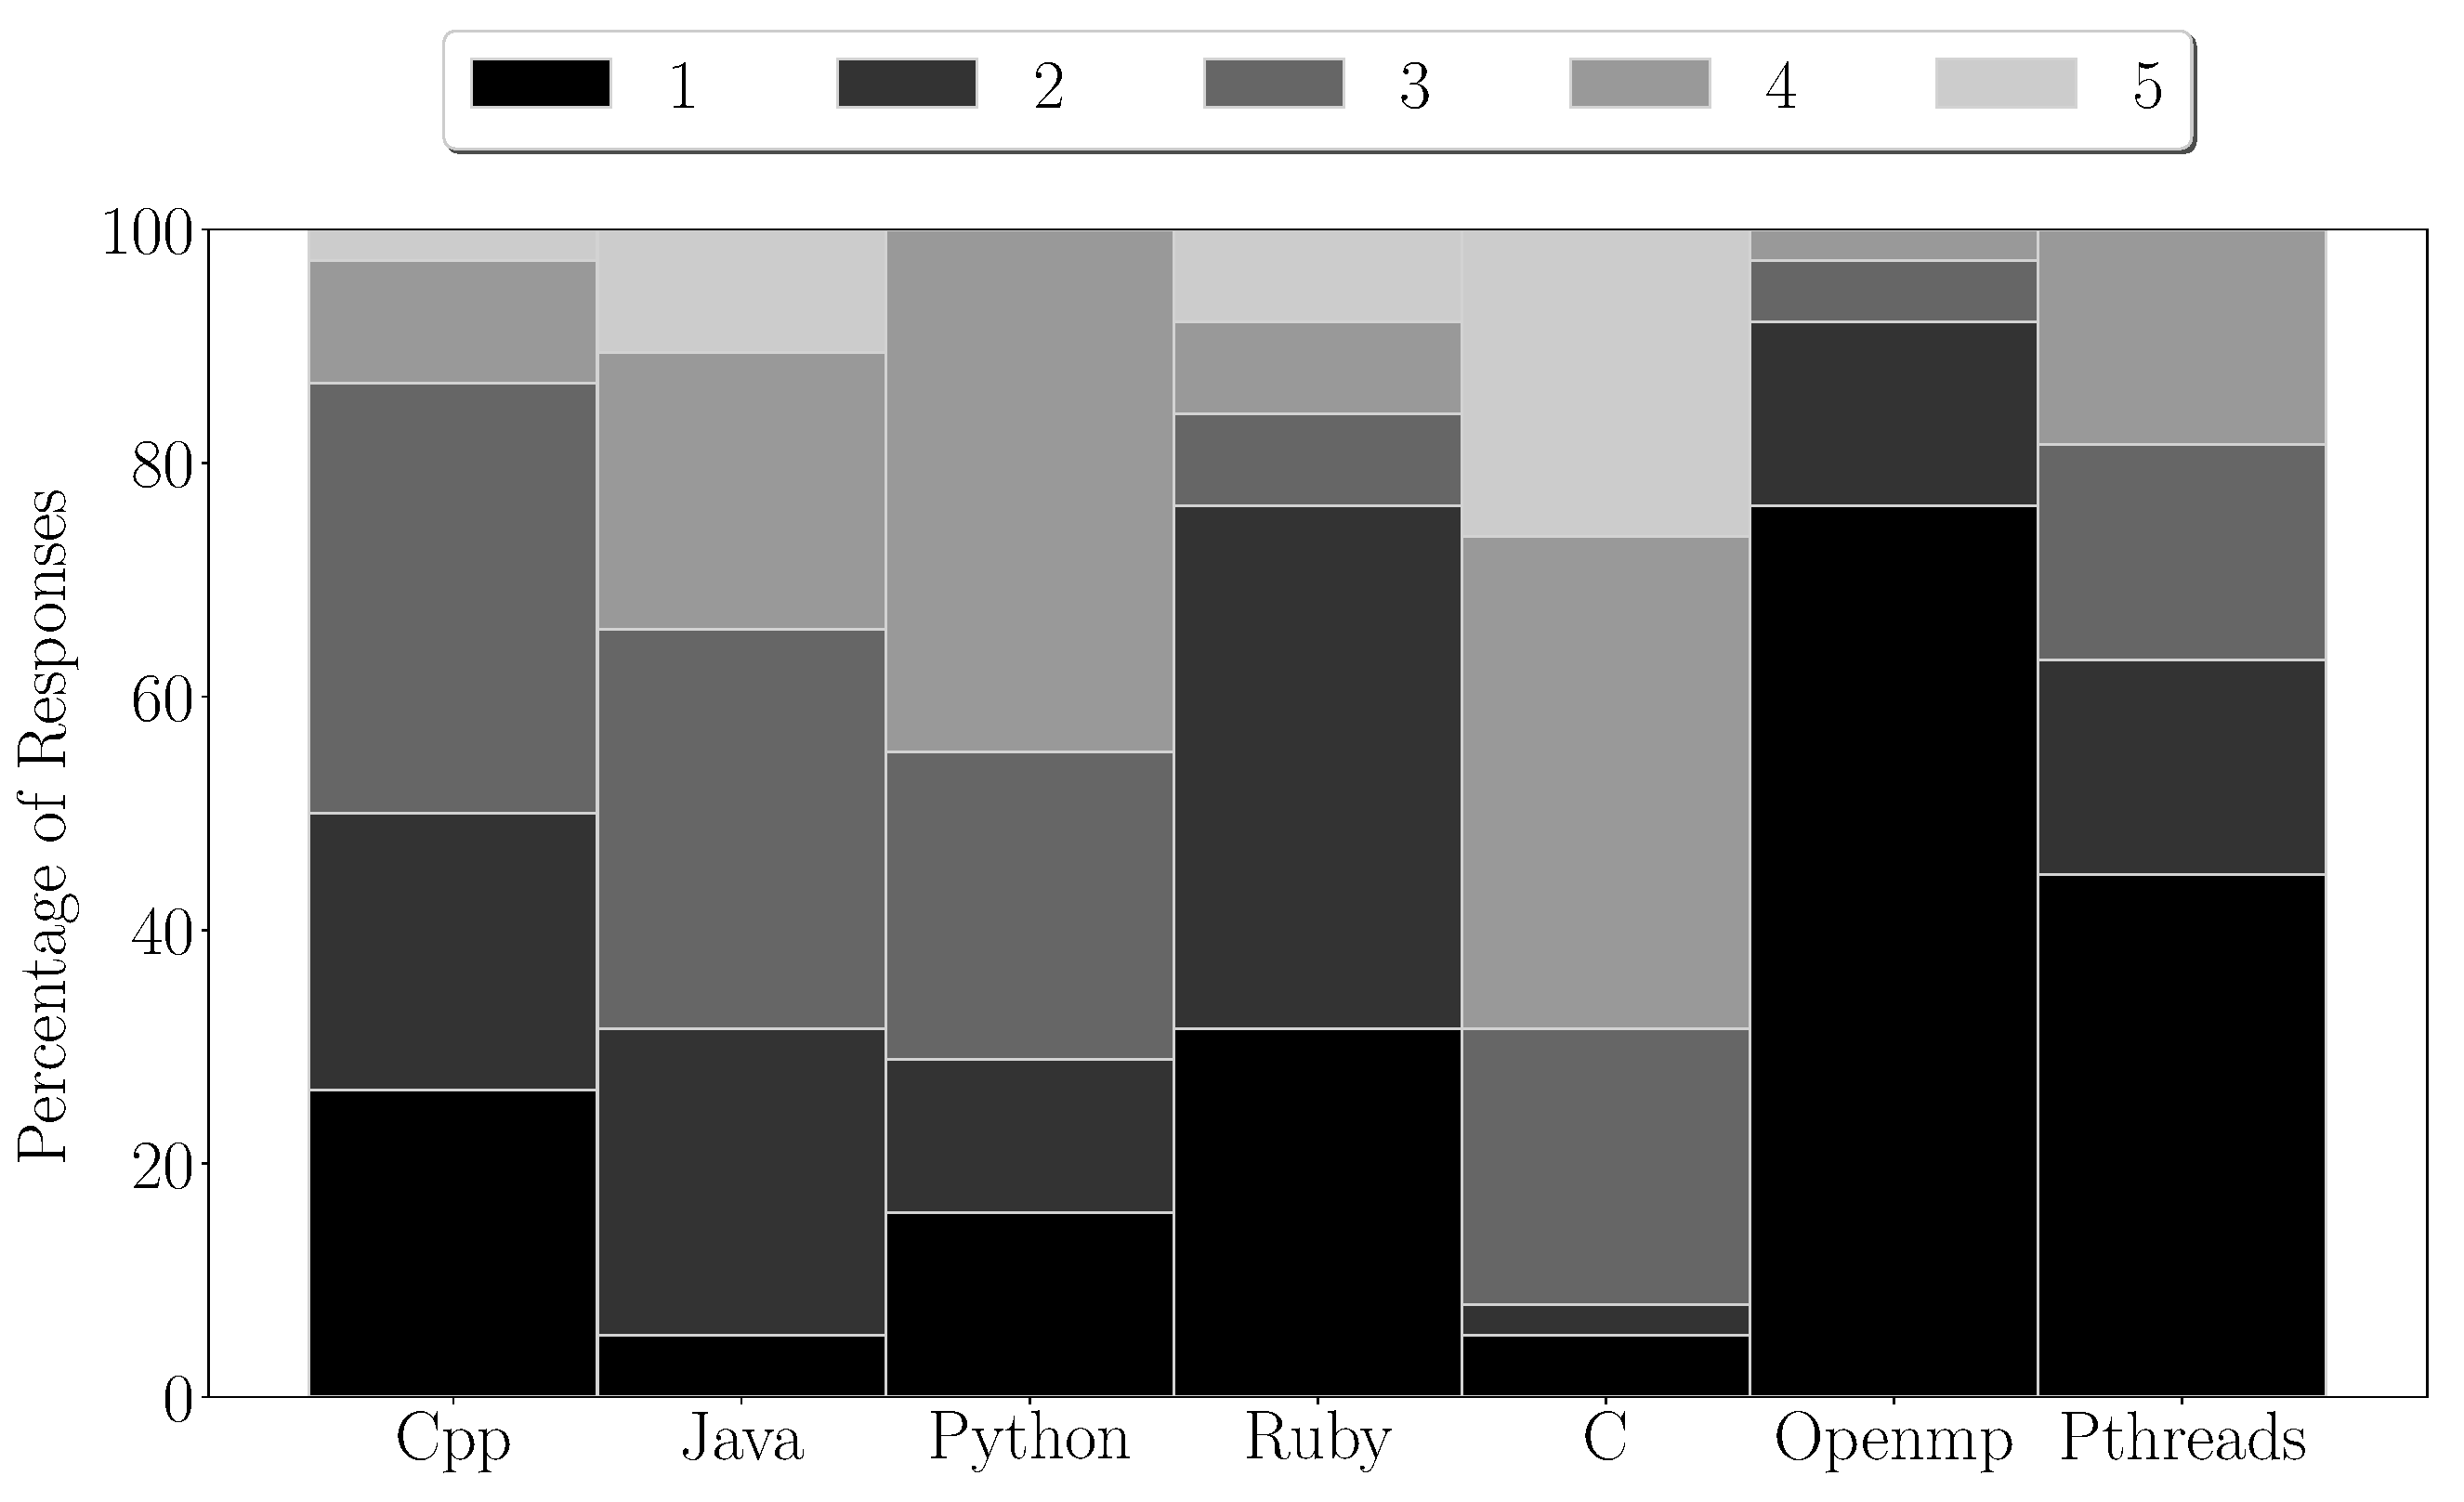
\includegraphics[width=0.85\columnwidth]{background_questions}
    \caption{Student knowledge \textit{before} the assignment}
    \label{fig:background}
\end{figure}

It is common for Computer Science introductory and advanced courses in the
graduate and undergraduate programs of the University of São Paulo to be given
in programming languages such as C, Java and Python. Figure
\ref{fig:background} shows that students reported higher proficiency in those
languages. The C language was the one with which students reported most
proficiency.

We asked the students to evaluate their proficiency in \textit{OpenMP} and
\textit{Pthreads}, \textit{before} completing the assignment, with two sets of
questions. The first set used the same five-point scale as the other background
questions and is also shown in Figure \ref{fig:background}. The students
reported significantly larger proficiency in \textit{Pthreads} than
\textit{OpenMP}, and the majority of the students reported they did not know
\textit{OpenMP} before the course.

\begin{table}[htpb]
    \centering
    \begin{tabular}{@{}p{0.9\columnwidth}p{0.08\columnwidth}@{}}
        \toprule
        \multicolumn{1}{c}{\scriptsize{Have you$\dots$}} & \textnumero \\ \midrule
        \scriptsize{Had contact with parallel and distributed concepts before?} & $(1)$ \\
        \scriptsize{Had contat with the APIs before?} & $(2)$ \\
        \scriptsize{Learned from the OpenMP class?} & $(3)$ \\
        \scriptsize{Learned from the Pthreads class?} & $(4)$ \\ \bottomrule
    \end{tabular}
    \caption{Questions for Figure \ref{fig:classes}}
    \label{tab:classes}
\end{table}

The second set of questions regarding student proficiency with the APIs
comprised the 4 \textit{Yes or No} questions listed in Table \ref{tab:classes}.
This set of questions also asked the students to evaluate whether the classes
on each subject helped their understanding and learning of the technologies.
The student responses for this set are shown in Figure \ref{fig:classes}.  The
majority of the students have had previous contact with the concepts related to
concurrent, parallel and distributed programming, but the majority also have
not had contact or experience with \textit{OpenMP} or \textit{Pthreads}.  Most
students reported that the classes on each API helped their learning.

\begin{figure}[htpb]
    \centering
    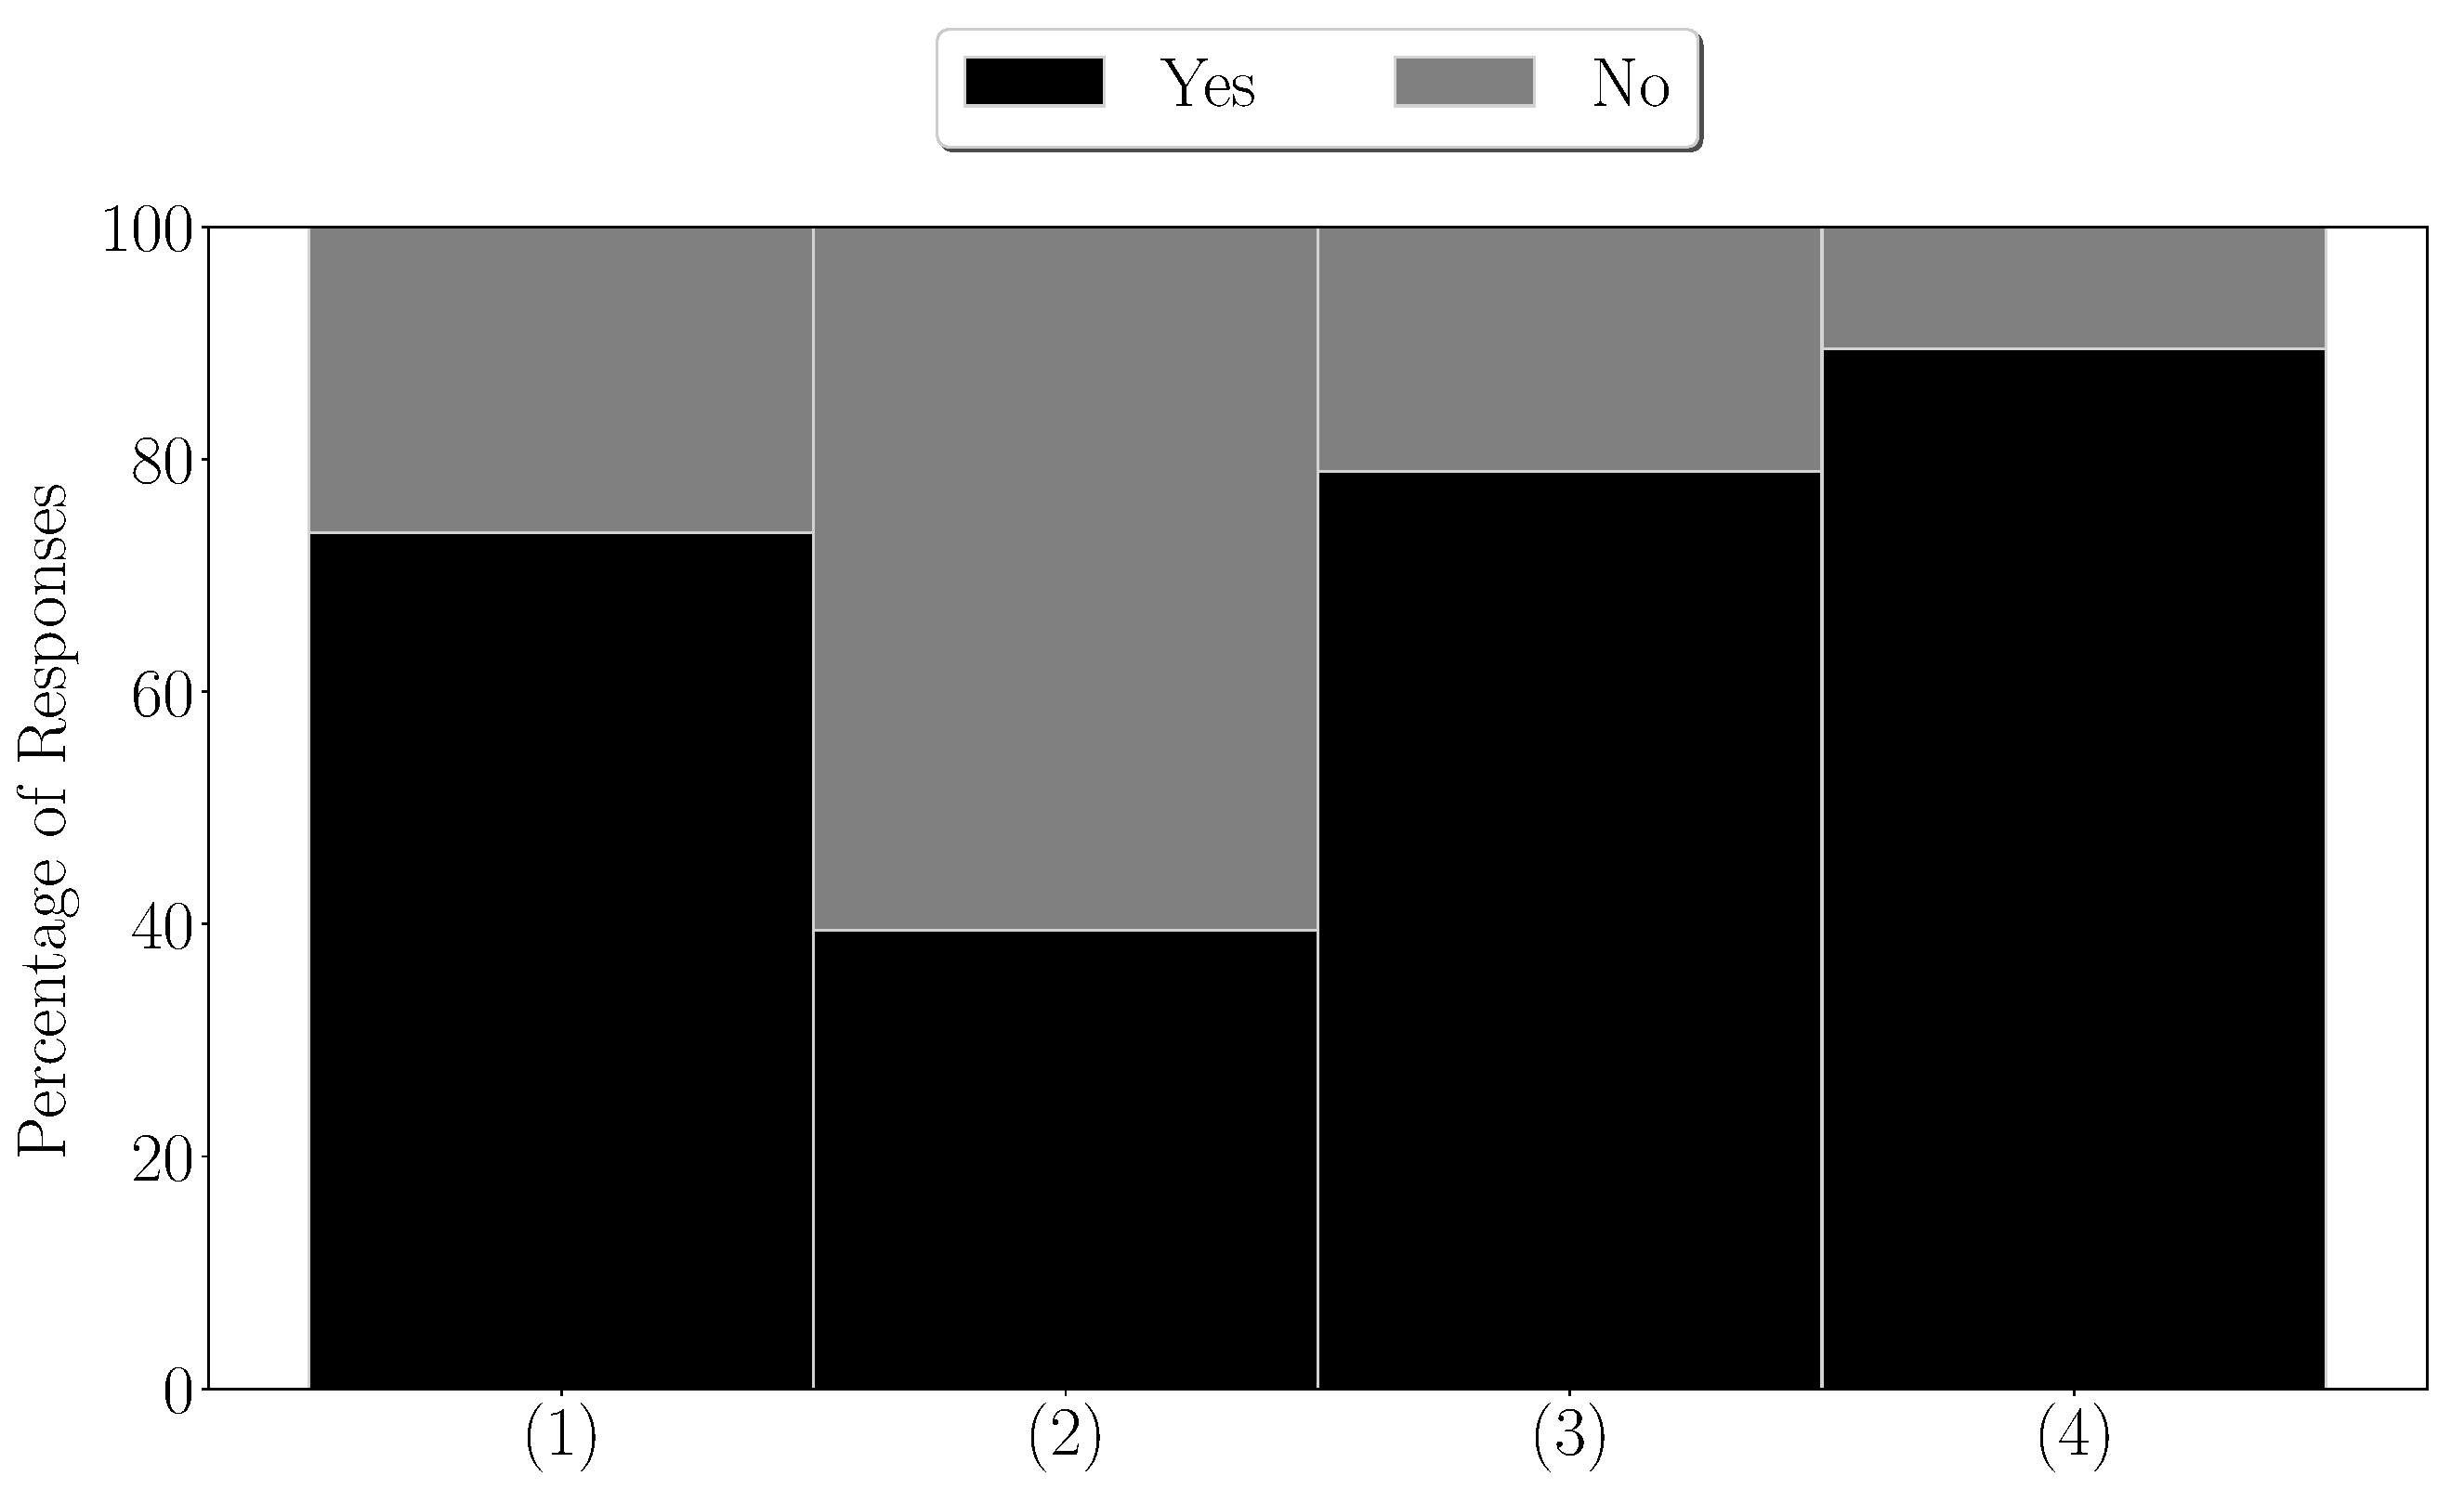
\includegraphics[width=0.85\columnwidth]{classes_questions}
    \caption{Student API knowledge \textit{before} the assignment and their relation to classes}
    \label{fig:classes}
\end{figure}

\subsection{Responses}

We asked the students to answer 3 sets of questions regarding their
experience with \textit{OpenMP} and \textit{Pthreads}, \textit{after}
completing the assignment.
The first set of questions used a Likert-type Scale to measure the relationship
of the students with the two APIs in the context of the assignment. The Likert
Scale~\cite{likert1932technique} enables respondents to express their agreement
or disagreement with specific statements. Respondents choose between five
options: \textit{Strongly Agree} (SA), \textit{Agree} (A), \textit{Neutral}
(N), \textit{Disagree} (D) and \textit{Strongly Disagree}.

The questions of the first set are listed in Table \ref{tab:likert}. The
students expressed their agreement or disagreement with statements related to
the difficulty of parallelizing the first loop with independent iterations,
parallelizing the two nested loops with independent iterations and improving
the performance of the sequential code. Each question was repeated for
\textit{OpenMP} and \textit{Pthreads}, in a total of $6$ questions.

\begin{table}[htpb]
    \centering
    \begin{tabular}{@{}p{0.7\columnwidth}p{0.1\columnwidth}p{0.05\columnwidth}@{}}
        \toprule
        \multicolumn{2}{c}{\scriptsize{It is easy to$\dots$}} & \textnumero \\ \midrule
        \multirow{2}{*}{\parbox{0.7\columnwidth}{\scriptsize{Parallelize loops with independent iterations using:}}} & \scriptsize{OpenMP} & $(1)$ \\
        & \scriptsize{Pthreads} & $(2)$ \\
        \addlinespace{}
        \multirow{2}{*}{\parbox{0.7\columnwidth}{\scriptsize{Parallelize nested loops with independent iterations using:}}} & \scriptsize{OpenMP} & $(3)$ \\
        &  \scriptsize{Pthreads} & $(4)$ \\
        \addlinespace{}
        \multirow{2}{*}{\parbox{0.7\columnwidth}{\scriptsize{Improve the performance of sequential code using:}}} & \scriptsize{OpenMP} & $(5)$  \\
        &  \scriptsize{Pthreads} & $(6)$ \\ \bottomrule
    \end{tabular}
    \caption{Likert-like Scale questions for Figure \ref{fig:likert}}
    \label{tab:likert}
\end{table}

Figure \ref{fig:likert} shows a visualization of the students' responses.  The
height of each stacked sub-column represents the percentage of respondents that
selected each of the correspondent Likert scale agreement levels, which are
represented by different colors.

\begin{figure}[htpb]
    \centering
    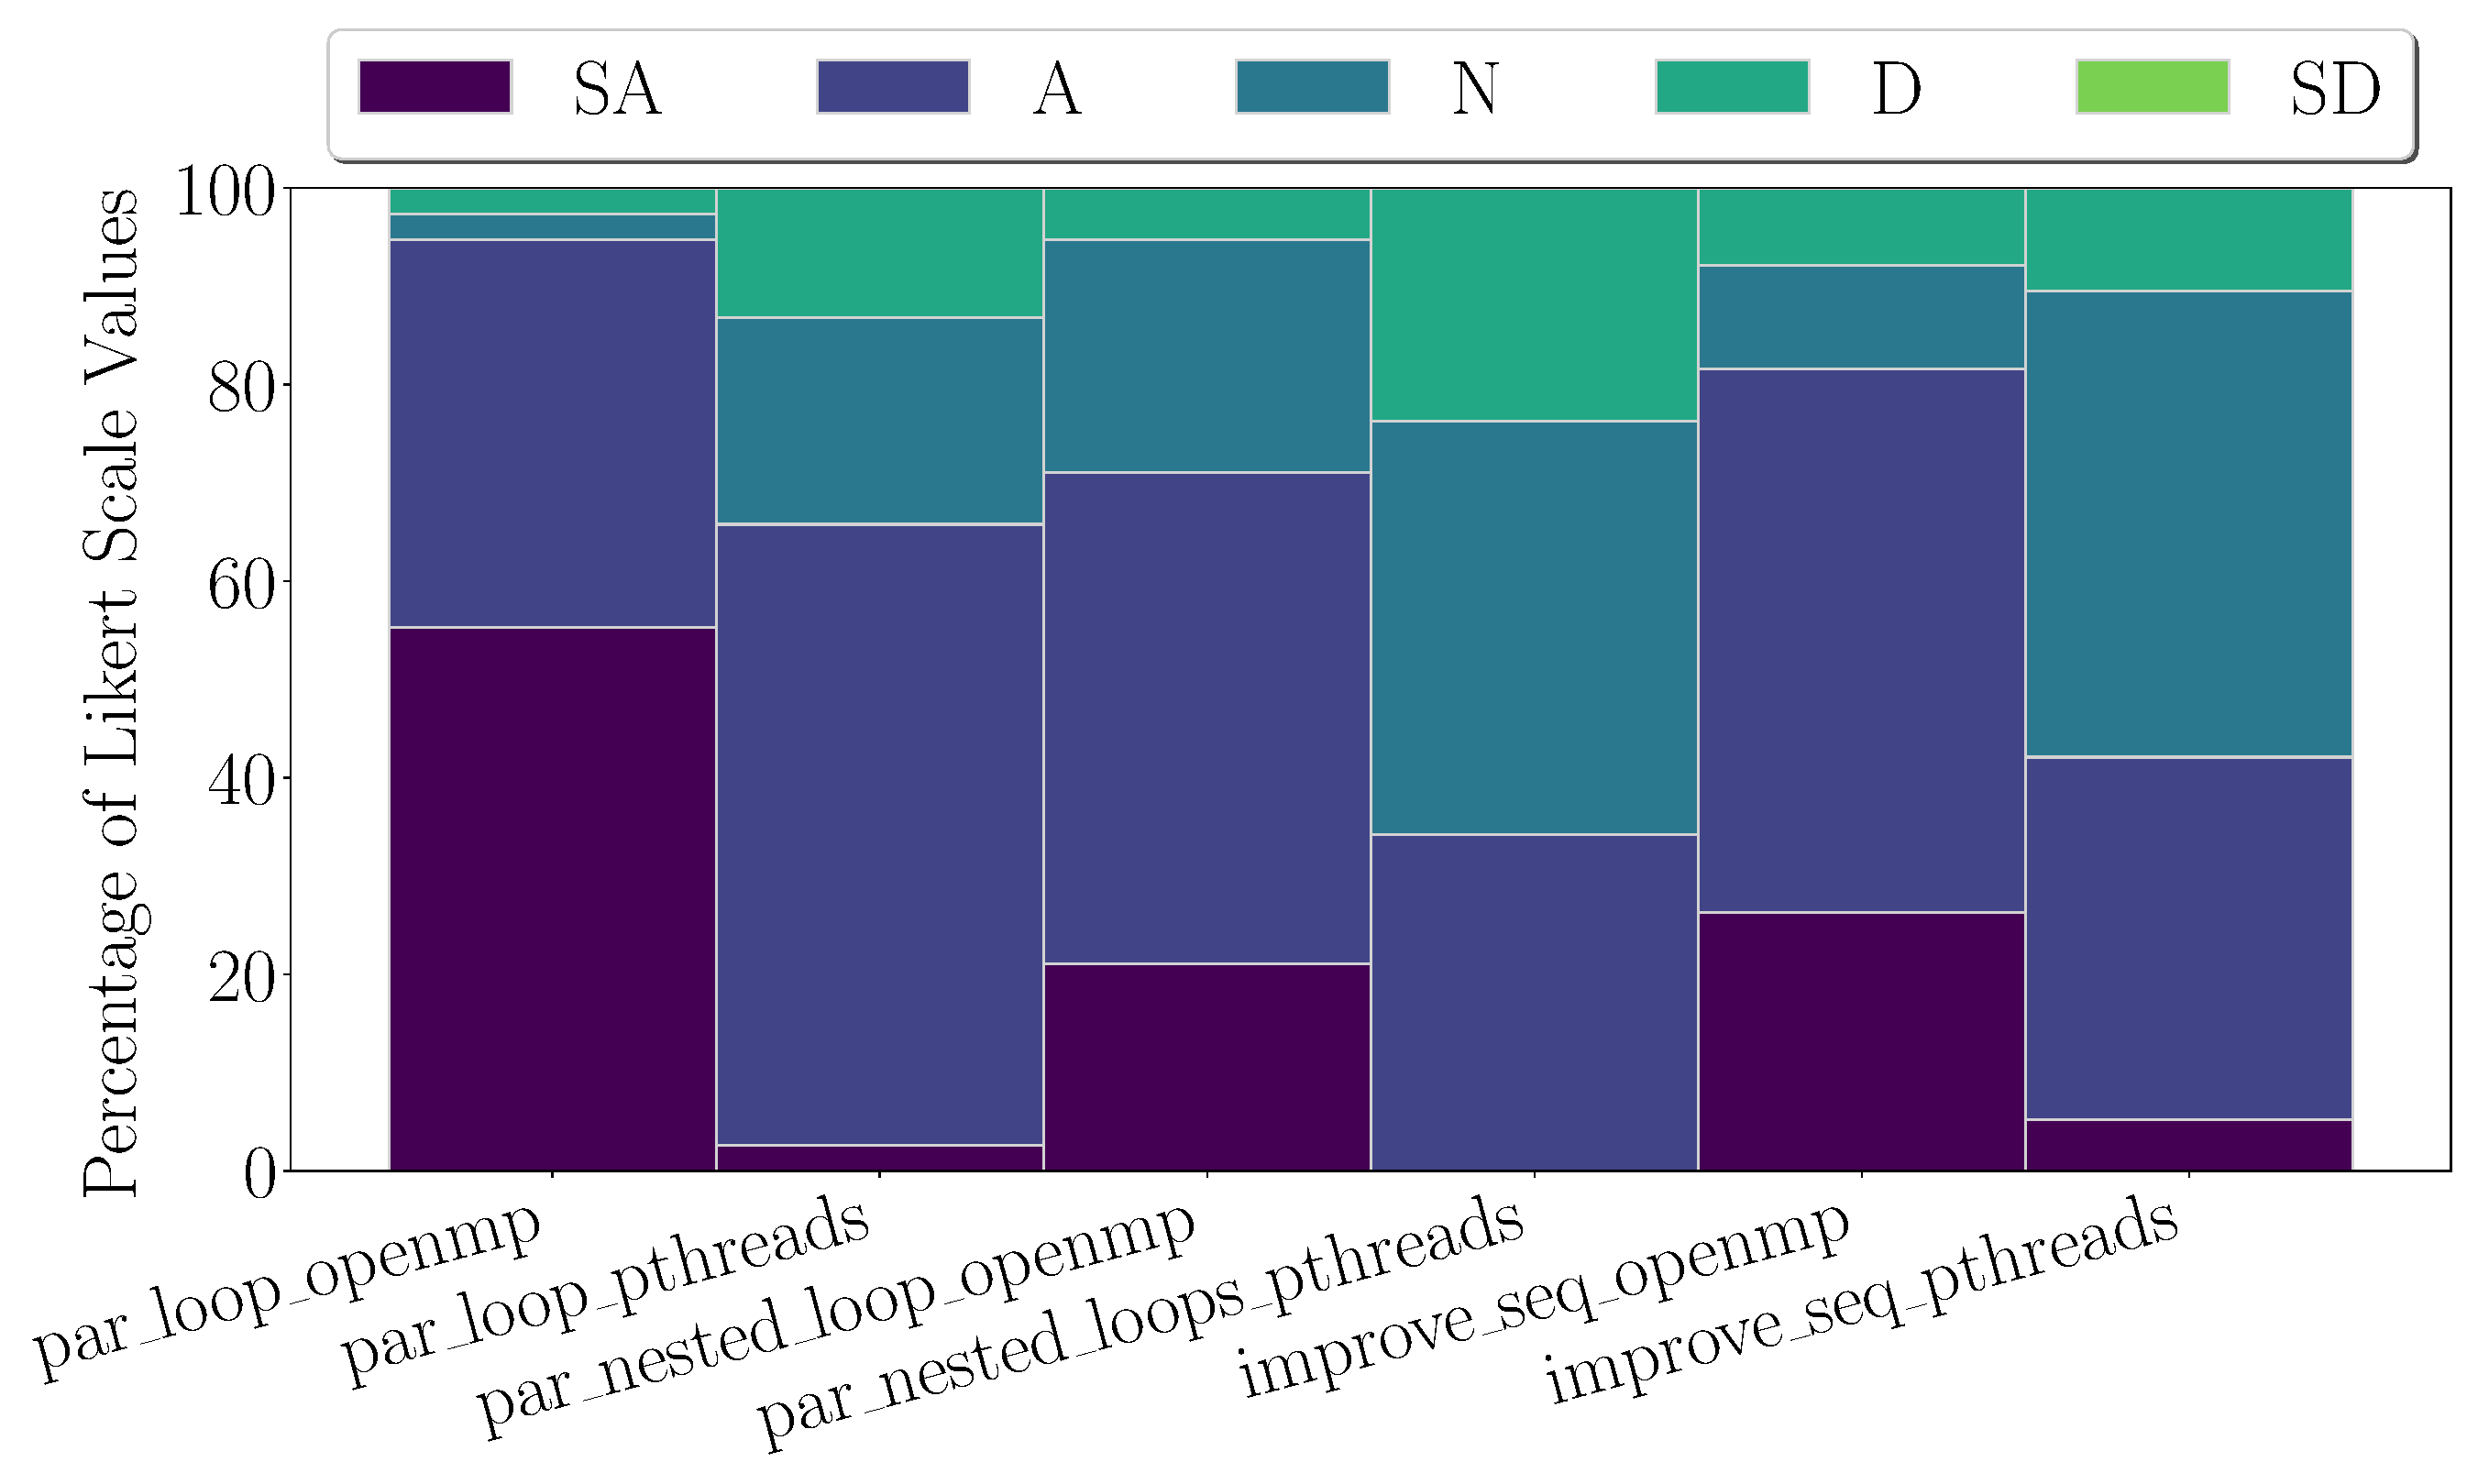
\includegraphics[width=0.85\columnwidth]{likert_questions}
    \caption{Student responses to the Likert Scale questions in Table \ref{tab:likert}}
    \label{fig:likert}
\end{figure}

The percentages of \textit{Strongly Agree} (SA) and \textit{Agree} (A)
responses are significantly larger for questions $(1)$, $(3)$ and $(5)$, which
are related to \textit{OpenMP}.  Likewise, the percentages of \textit{Disagree}
(D) responses are significantly larger for questions $(2)$, $(4)$ and $(6)$,
which are related to \textit{Pthreads}. These responses lead to the conclusion
that \textbf{the perception of the students was that it was easier to use
\textit{OpenMP} than \textit{Pthreads}} to parallelize and improve the
performance of the sequential code provided in the assignment.

The second set of questions used a five-point scale to measure the difficulty
the students had with the learning process of the two APIs for the assignment.
Respondents expressed their difficulty to learn \textit{OpenMP} and
\textit{Pthreads} in a scale of $1$ to $5$, choosing a point between \textit{No
Difficulty} $(1)$ and \textit{Much Difficulty} $(5)$.

Figure \ref{fig:learning} shows a visualization of the students' responses.
The height of each stacked sub-column represents the percentage of respondents
that selected each of the correspondent difficulty levels, which are
represented by different colors.

\begin{figure}[htpb]
    \centering
    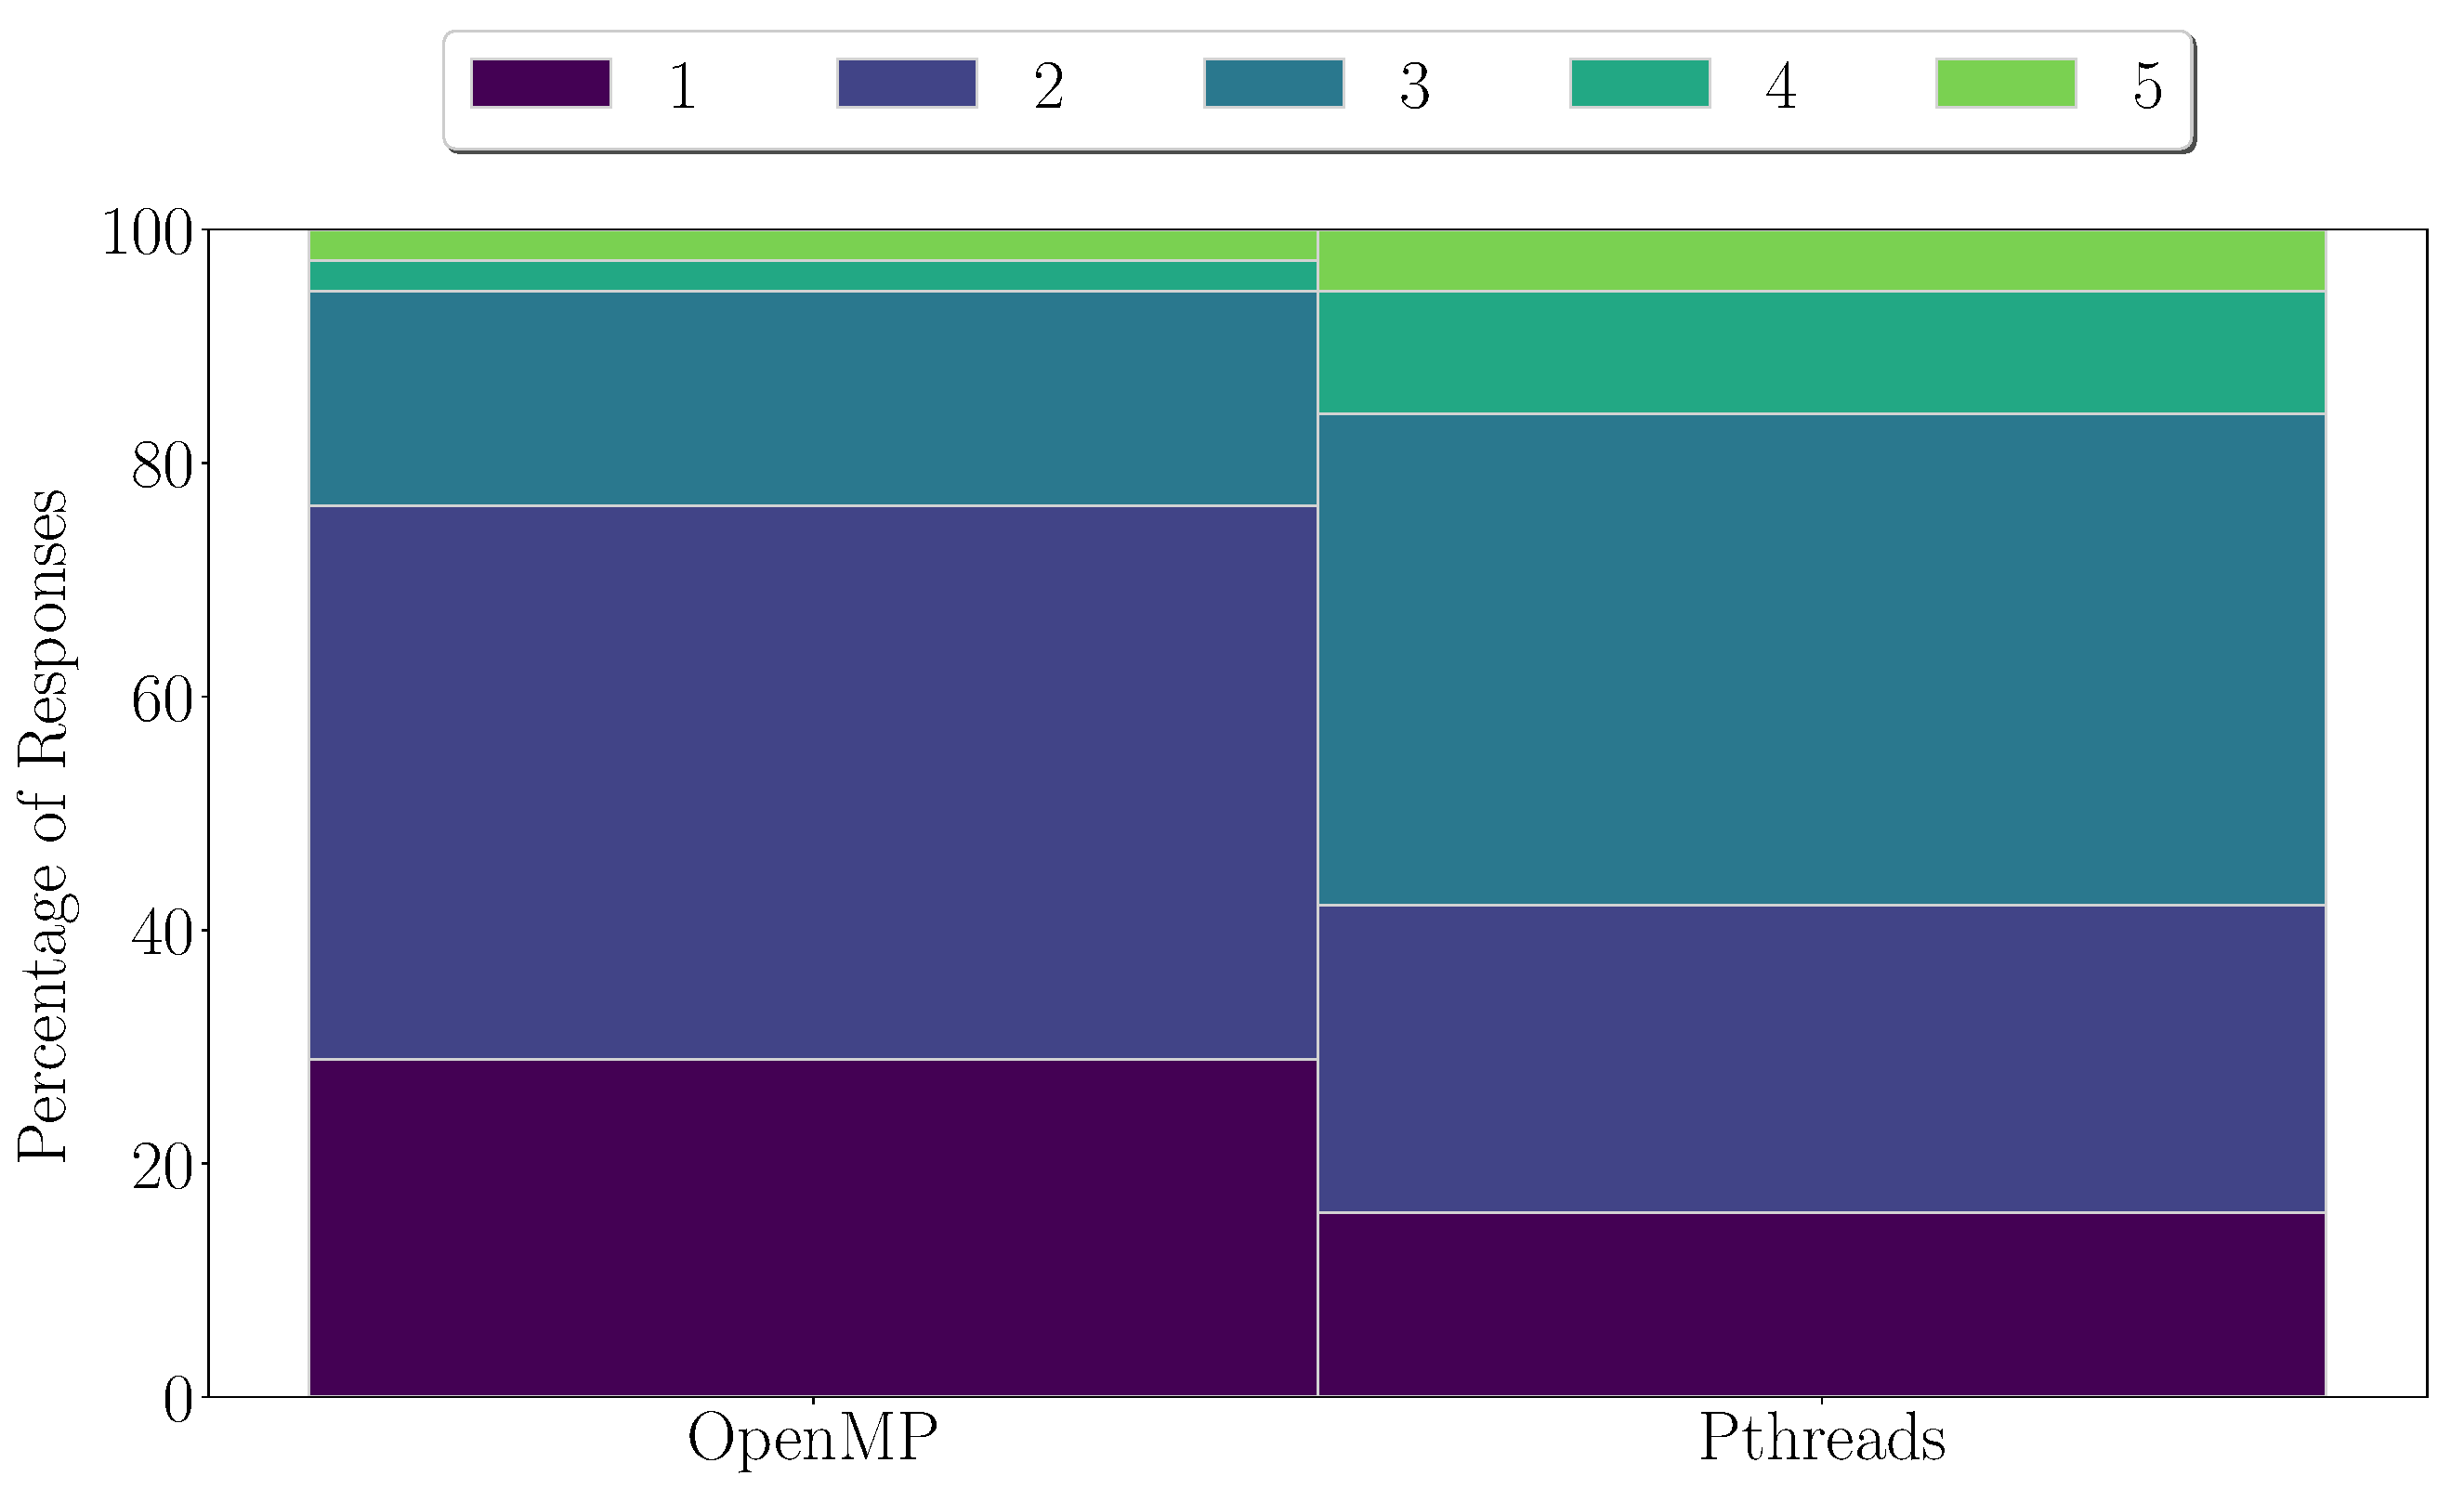
\includegraphics[width=0.85\columnwidth]{learning_difficulty_questions}
    \caption{Student difficulty to learn the APIs in a five-point scale}
    \label{fig:learning}
\end{figure}

The percentages of \textit{No Difficulty} $(1)$ and difficulty level $(2)$
responses are significantly larger for learning \textit{OpenMP}. Likewise, the
percentages of difficulty level $(4)$ and \textit{Much Difficulty} $(5)$
responses are significantly larger for learning \textit{Pthreads}.  We derive
from these responses the conclusion that \textbf{the students perceived less
difficulty to learn \textit{OpenMP} than \textit{Pthreads}} for the purposes of
the assignment.

The final set of questions regarding the usage and learning of \textit{OpenMP}
and \textit{Pthreads} in the context of the first assignment presented
comparison questions between the two APIs. Students chose which API they
perceived was the best answer to the questions in Table \ref{tab:comparisons}.

Responses to question $(13)$ in Table \ref{tab:comparisons} were not obtained
directly from the students. We analysed each assignment submission and
evaluated the performance of the each solution across the specified
experimental settings.

\begin{table}[htpb]
    \centering
    \begin{tabular}{@{}p{0.9\columnwidth}p{0.08\columnwidth}@{}}
        \toprule
        \multicolumn{1}{c}{\scriptsize{Which technology$\dots$}} & \textnumero \\ \midrule
        \scriptsize{Was more difficult to learn?} & $(7)$ \\
        \scriptsize{Was simpler to use?} & $(8)$ \\
        \scriptsize{Was easier to use?} & $(9)$ \\
        \scriptsize{Was easier to use for parallelizing loops with independent iterations?} & $(10)$ \\
        \scriptsize{Was easier to use for parallelizing nested loops with independent iterations?} & $(11)$  \\
        \scriptsize{Was easier to use for improving the performance of a sequential program?} & $(12)$  \\
        \scriptsize{Had the best performance on your assignment?} & $(13)$ \\ \bottomrule
    \end{tabular}
    \caption{Questions for Figure \ref{fig:comparisons}}
    \label{tab:comparisons}
\end{table}

Figure \ref{fig:comparisons} shows a visualization of the students' responses.
The height of each stacked sub-column represents the percentage of respondents
that selected each API, which are represented by different colors.

The percentage of \textit{OpenMP} selections is significantly larger for all
questions, except for questions $(7)$ and $(13)$. The responses for questions
$(7)$ -- $(12)$ strengthen the previous conclusion that the perception of the
students was that it was easier to use \textit{OpenMP} than \textit{Pthreads}
in the context of the assignment. The performance results that we obtained from
analysing the students' submissions challenge the perception of the students.
The responses to question $(13)$, extracted by our analysis, show that
\textbf{the students achieved better performance when using \textit{Pthreads}
than \textit{OpenMP}}.

\begin{figure}[htpb]
    \centering
    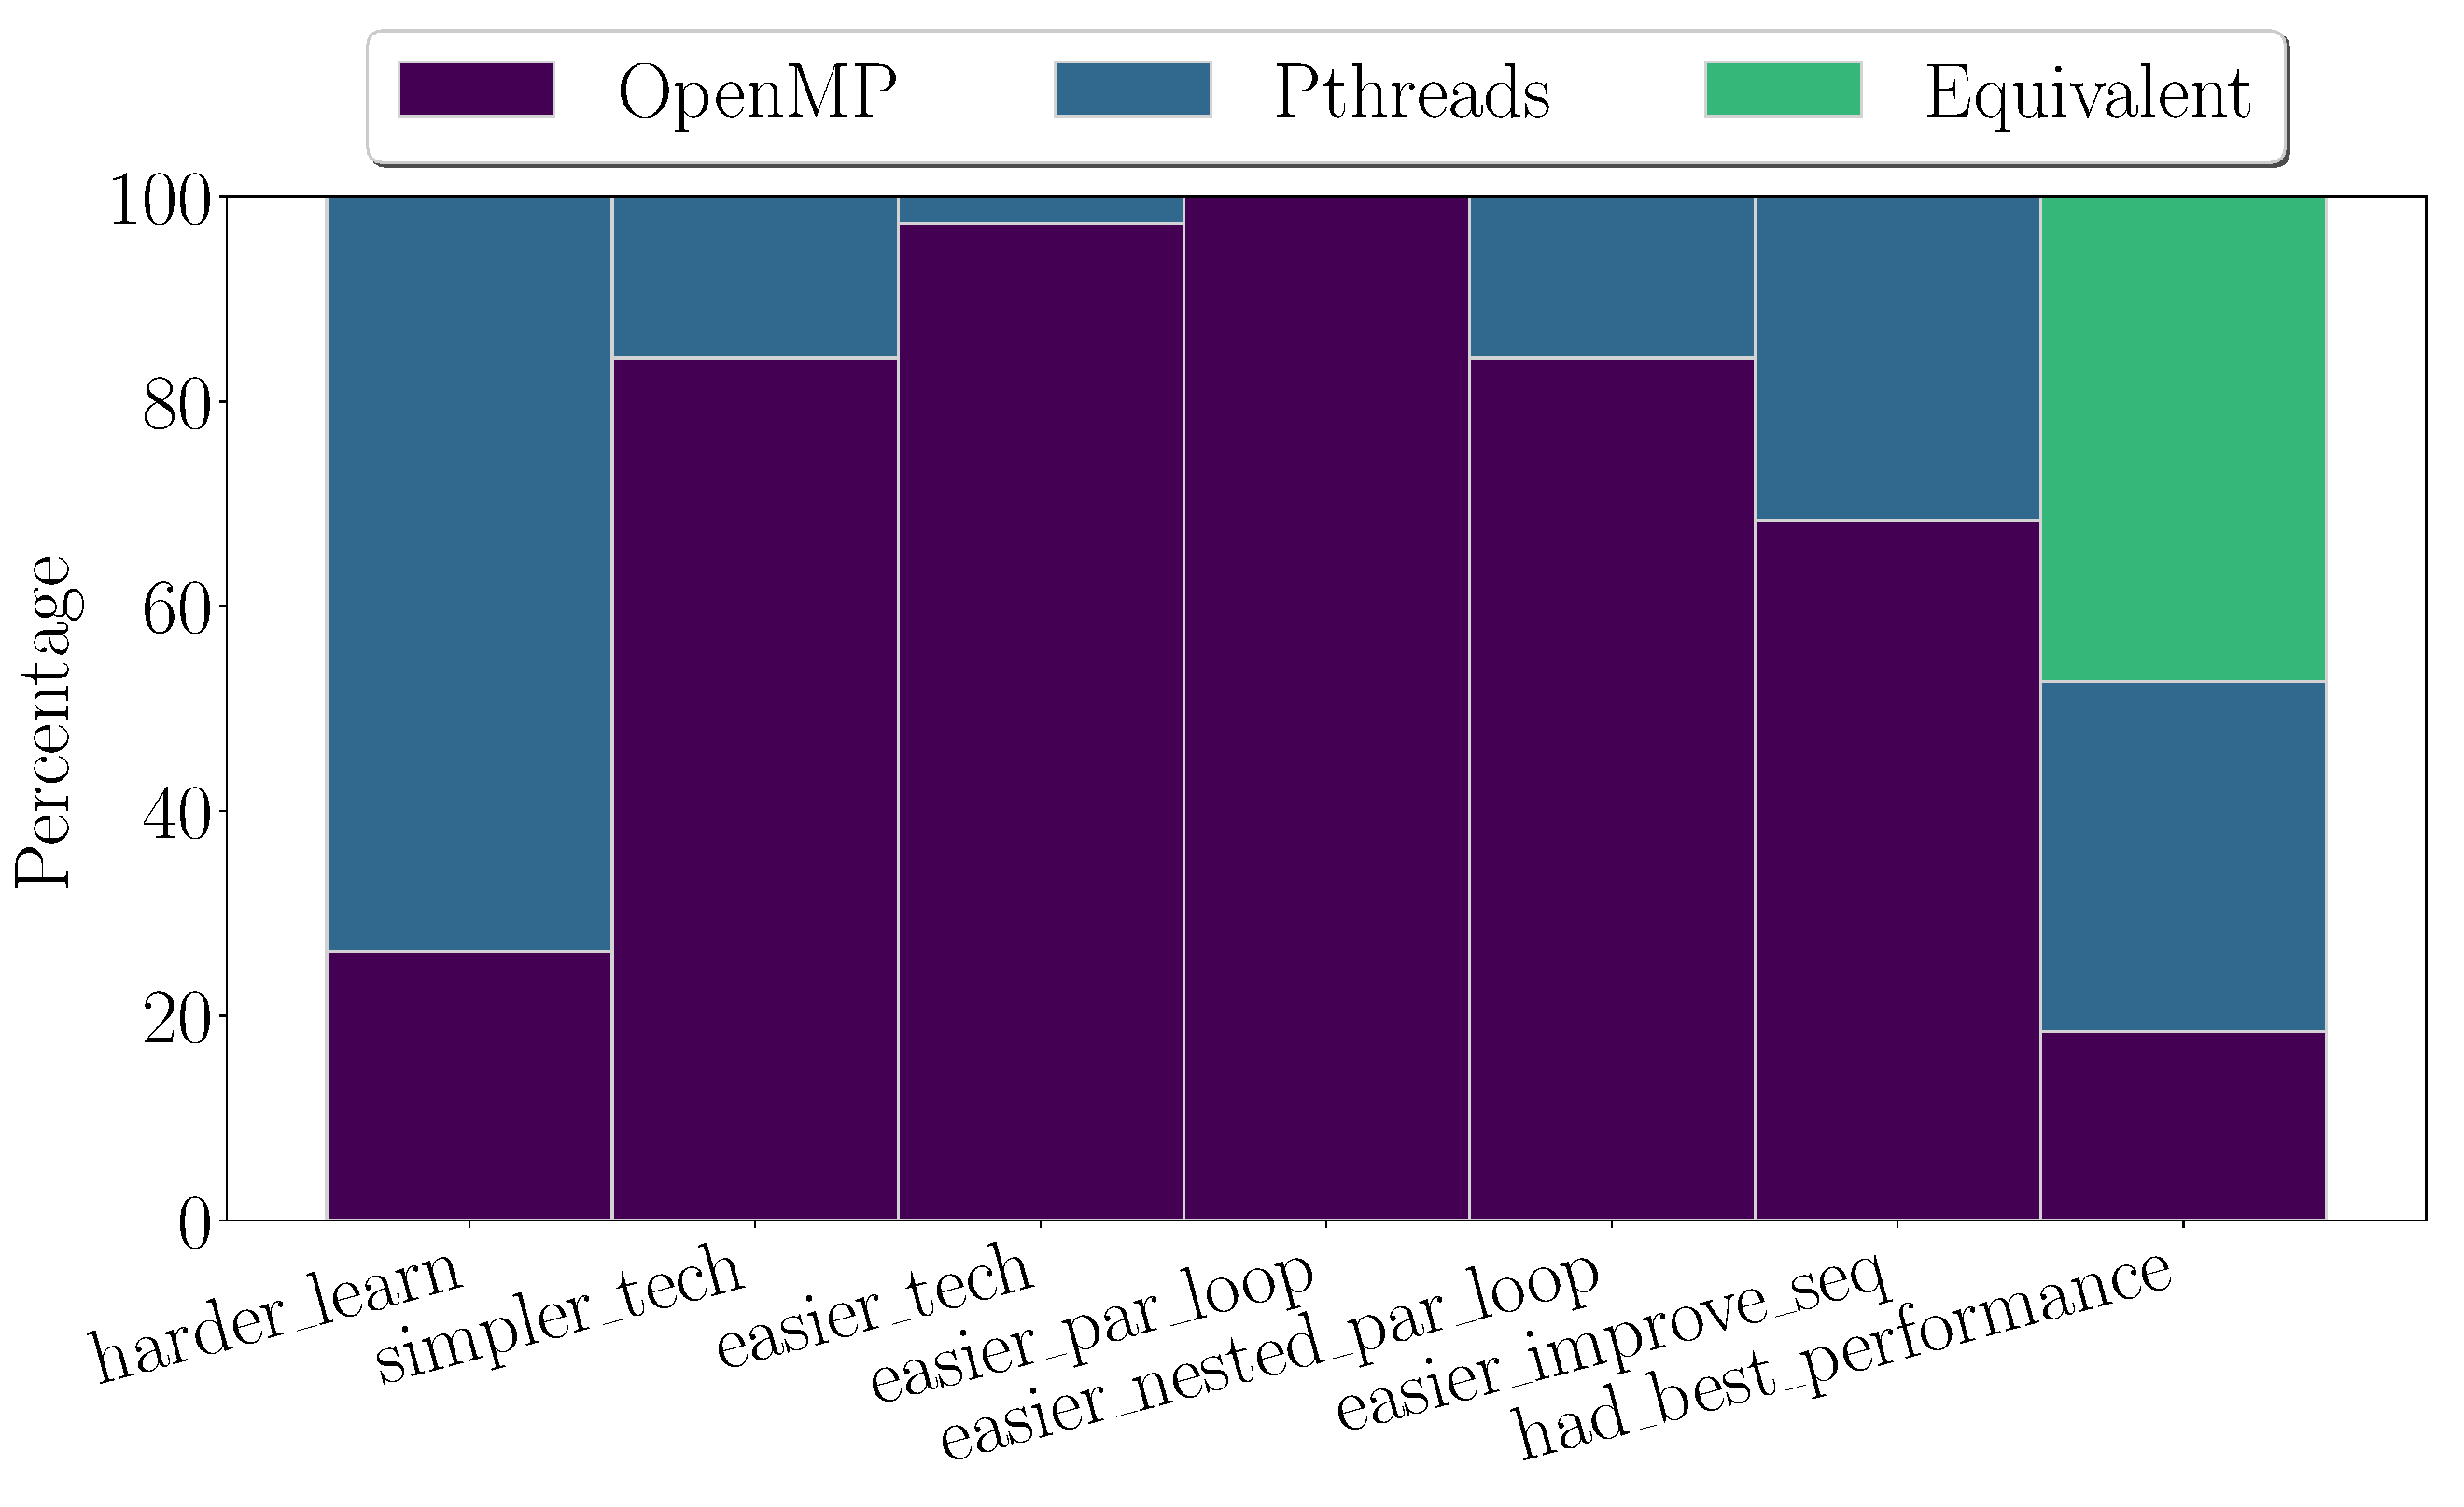
\includegraphics[width=0.85\columnwidth]{comparisons}
    \caption{Student responses to the questions in Table \ref{tab:comparisons}}
    \label{fig:comparisons}
\end{figure}

\todo[inline,color=cyan,author=Pedro]{Improve these last paragraphs}

The responses presented in this section enable the conclusion that the students
perceived less difficulty using and learning \textit{OpenMP} in the context
of the assignment. They also reported the perception that using \textit{OpenMP}
made it easier to improve the performance of the sequential code we provided.
Our analysis of the submissions revealed that the majority of the students
($52.2\%$) achieved better performance in the assignment with either
\textit{OpenMP} ($17.4\%$) or \textit{Pthreads} ($34.8\%$). Contradicting the
perception of the students, the implementation using \textit{Pthreads} achieved
better performance in twice the submissions.

This shows that the perceptions of usability and performance improvement
regarding \textit{OpenMP} did not reflect in the actual implementations and
submissions. We believe that \textit{OpenMP} is still not as easy as it appears
to be, and that the students' responses strengthen the argument for teaching
lower-level technologies for parallel and distributed computing.

\section{Lessons Learned}
\label{sec:lessons}

TO-DO ...

\section{Conclusions}
\label{sec:conclusions}

TO-DO ...

%---
\section*{Acknowledgments}
\label{sec:acknowledgments}

The authors would like to thank Students who participated in this exercise ...


%---

\bibliographystyle{ACM-Reference-Format}
\bibliography{references}

\end{document}
